\DiaryEntry{Cubic Equations - in progress}{2018-03-05}{Complex Analysis}


Based / inspired by Tristan Needdham, "Visual Complex Analysis".


We want to solve the cubic equation

\bee
y = x^3 + a x^2 + b x + c = 0
\eee

The inflection point (that is where $y'' = 0$) is given by: $y' = 3x^2 + 2ax + b, y'' = 6x + 2a$ and from this follows that the inflection point is $x = -a / 3$. Exercise V/1 in the book is to show that the quadratic term of the equation above vanishes when we substitute $x \rightarrow u - a_0/3$. We can simply perform the substitution and arrive at 

\bee
y = (u-a/3)^3 + a(u-a/3)^2 + b(u-a/3) + c = \cdots + u^3 + Bu + C
\eee

where $A,B,C$ are some constants calculated via e.g. Maxima as follows.

\begin{verbatim}
(%i1)	ratsimp((u-a/3)^3+a*(u-a/3)^2 + b*(u-a/3) + c);
(%o1)	(27*u^3+(27*b-9*a^2)*u+27*c-9*a*b+2*a^3)/27
\end{verbatim}

This shows that we only have to deal with equations with $a=0$. For whatever reasons, we write these equations as

\be
\label{2018-03-05:eq1}
y = x^3 - 3px - 2q
\ee

As a general note, either there are three real solutions, or one real solution and two complex (conjugate) ones. A special case is that there is one (three-fold) real solution.


\subsection{Simple Cases}

Consider first the case when $q=0$.

\bee
y = x^3 - 3px = 0
\eee

which we can factor as $y = x(x^2 - 3p) = 0$ and we have the three solutions $x_0 = 0, x_{1,2} = \pm \sqrt{3p}$.

The curve fulfills the following symmetry: $y(-x) = -y(x)$.

We can see more clearly what happens by calculating the position of local minimums and maximums. Assume that $p>0$, $y' = 3x^2 - 3p = 0$ and therefore $x = \pm \sqrt{p}$. With $y'' = 6x$, $y''(\sqrt{p}) > 0$ and therefore $x = \sqrt{p}$ is a local minimum. We have $y''(-\sqrt{p}) < 0$ and therefore $x = -\sqrt{p}$ is a local maximum. For large absolute values of $x$, the cubic term dominates.

The following plot shows $y=x^3 - 12x$: The local maximum and minimum are located at $\pm2$, the zeros are $\pm 2 \sqrt{3}$. For large absolute values of $x$, the curve behaves like $x^3$.

\begin{figure}[H]
	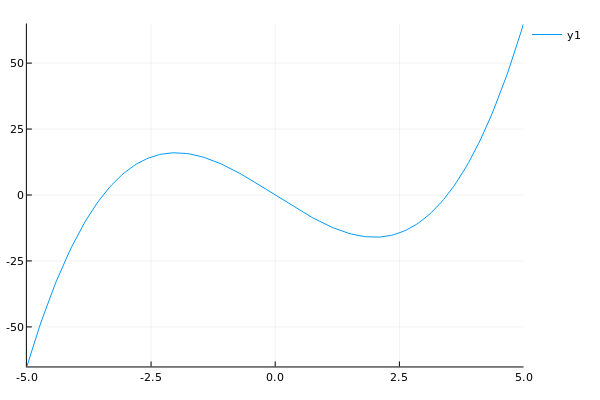
\includegraphics[scale=0.7]{images/cubic_01.png}
\end{figure}

\subsection{Complete Solution}

In exercise V/2, a solution to \eqref{2018-03-05:eq1} is calculated. We start with an Ansatz $x = s+t$. We show that $x$ solves \eqref{2018-03-05:eq1} when $st=p$ and $s^3 + t^3 = 2q$: Inserting into $x^3 = 3px + 2q$ we obtain

\bee
(s+t)^3 = 3st(s+t) + s^3 + t^3
\eee

Expanding the LHS, we see that this equation holds. \qed

We now express $t$ in terms of $s$ via $st=p \rightarrow t = p/s$ and insert this into $s^3 + t^3 = 2q \rightarrow s^3 + \frac{p^3}{s^3} = 2q$. This can be expressed as $s^6 + p^3 = 2qs^3$ and we obtain the equation

\bee
s^6 -2qs^3 + p^3 = 0
\eee

Setting $u = s^3$ we get $u^2 - 2qu + p^3 = 0$ which has the following two solutions

\bee
u_{1,2} = q \pm \sqrt{q^2 - p^3}
\eee

and back-substituting, we obtain

\bee
s = \sqrt[3]{q \pm \sqrt{q^2 - p^3}}
\eee

We can calculate $t^3 = 2q - s^3 = 2q - (q \pm \sqrt{q^2 - p^3}) = q \mp \sqrt{q^2 - p^3}$. From this follows $t = \sqrt[3]{q \mp \sqrt{q^2 - p^3}}$ and we finally have

\be
\label{2018-03-05:eq2}
x = s+t = \sqrt[3]{q \pm \sqrt{q^2 - p^3}} + \sqrt[3]{q \mp \sqrt{q^2 - p^3}}
\ee

We next observe that a cubic root has three solutions.

\paragraph{Cubic Roots.} We have a complex number $z = r e^{j \theta + 2m\pi}$ with $m$ being an integer. We seek another complex number $u = Re^{j\phi}$ whose third power equals $z$:

\bee
u^3 = z \rightarrow R^3e^{j3\phi} = r e^{j \theta + 2m\pi}
\eee

From this follows $R^3 = r \rightarrow R = \sqrt[3]{r}$ and $\phi = \frac{\theta +2m\pi}{3}$ and so the complex roots $z_m$ become

\bee
z_m = \sqrt[3]{r} e^{j(\theta + 2m\pi)/3}, \quad m=0,1,2
\eee

Currently open is the question, how we consistently get three solutions out of \eqref{2018-03-05:eq2}...


\subsection{Examples}

\paragraph{First example} is $x^3 - 6x - 6 = 0$. We have $p=2, q=3$ and blindly inserting into \eqref{2018-03-05:eq2} yields

\bee
x = \sqrt[3]{3 \pm \sqrt{9-8}} + \sqrt[3]{3 \mp \sqrt{9-8}} = \sqrt[3]{3 \pm 1} + \sqrt[3]{3 \mp 1} = \sqrt[3]{4} + \sqrt[3]{2} \approx 2.847
\eee

\begin{verbatim}
(%i8)	fpprintprec:4;
(fpprintprec)	4
(%i9)	allroots(x^3 - 6*x - 6);
(%o9)	[x=0.2836*%i-1.424,x=-0.2836*%i-1.424,x=2.847]
\end{verbatim}

In order to obtain the other two (conjugate complex) roots,  we need to consider complex results of $\sqrt[3]{4}$ and $\sqrt[3]{2}$, respectively. Assume we have $C^3 = A$ with $A$ positive. If $\sqrt[3]{A} = C$, then the two other solutions are $\left(-\frac{1}{2} \pm \frac{1}{2}\sqrt{3}j\right)C$.

Therefore, 4 other solution candidates are

\begin{align*}
&\left(-\frac{1}{2} + \frac{1}{2}\sqrt{3}j\right) \sqrt[3]{4} + \left(-\frac{1}{2} + \frac{1}{2}\sqrt{3}j\right) \sqrt[3]{2} \approx -1.424 + 2.466j\\
&\left(-\frac{1}{2} - \frac{1}{2}\sqrt{3}j\right) \sqrt[3]{4} + \left(-\frac{1}{2} + \frac{1}{2}\sqrt{3}j\right) \sqrt[3]{2} \approx -1.424 + 0.2836j \\
&\left(-\frac{1}{2} + \frac{1}{2}\sqrt{3}j\right) \sqrt[3]{4} + \left(-\frac{1}{2} - \frac{1}{2}\sqrt{3}j\right) \sqrt[3]{2} \approx -1.424 + 0.2836j \\
&\left(-\frac{1}{2} - \frac{1}{2}\sqrt{3}j\right) \sqrt[3]{4} + \left(-\frac{1}{2} - \frac{1}{2}\sqrt{3}j\right) \sqrt[3]{2} \approx -1.424 - 2.466j
\end{align*}

However, note that valid solutions also need to fulfill $st=p$. This removes the first and fourth candidate, leaving the following three solutions:

\bee
2.847, -1.424 + 0.2836j, -1.424 - 0.2836j
\eee

which is in line with the Maxima solution.

\paragraph{Second example} is $x^3 - 4x + 1 = 0$. We have $p=4/3, q=-1/2$ and blindly inserting into \eqref{2018-03-05:eq2} yields

\bee
x = \sqrt[3]{-\frac{1}{2} \pm \sqrt{\frac{1}{4}-\frac{64}{27}}} + \sqrt[3]{-\frac{1}{2} \mp \sqrt{\frac{1}{4}-\frac{64}{27}}}
\eee

The value in the square roots is negative; i.e. the result is imaginary. The argument of the cubic root is then a complex number and so is the result. However, the imaginary parts seem to cancel each other out, leaving three real solutions.

\begin{verbatim}
(%i8)	fpprintprec:4;
(fpprintprec)	4
(%i15)	allroots(x^3 - 4*x +1);
(%o15)	[x=0.2541,x=1.861,x=-2.115]
\end{verbatim}